\section{Definitions}

\textbf{CGN} \textit{(Convolutional Graph Neural Network)} --- A type of GNN which generalizes the convolution operation to graphs.
Often we encounter convolution while we work with grid-structured data like images, but here we use same idea (aggregate features of the neighbors) on nodes instead of pixels\cite{9046288}.

\begin{figure}[h]
    \begin{multicols}{2}
        \centering
        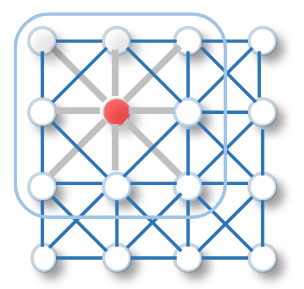
\includegraphics[width=0.25\textwidth]{conv.png}
        \caption{Convolution on image}
    
        \centering
        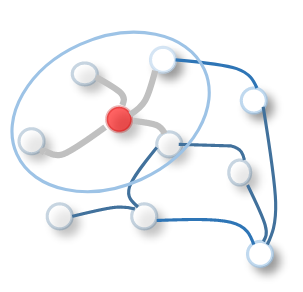
\includegraphics[width=0.25\textwidth]{CGN_conv.png}
        \caption{Convolution on graph}
    \end{multicols}
\end{figure}

\textbf{GAT} \textit{(Graph attention network)} --- A type of GNN which uses attention mechanism (also borrowed from `casual' neural networks) which allows us to work with inputs of variable sizes and to focus on the most important features~\cite{velickovic2018graph}. 
